% Chapter 3 - Some important points
%==========================
In this section, the details of the framework are presented. It consists of three major modules: \emph{Region-Category Interaction Encoder}, \emph{Hierarchical Recurrent Framework} and \emph{Attention Mechanism}. These three modules will be explained in detail in the following subsections. The model architecture is presented in Figure \ref{fig:framework}, where the output of one layer serves as the input to the next one.

\section{Category Dependency Encoder}
To consider the geographical context of regions, the POI information is incorporated into the process of generating the region
embedding vector. Formally, the constraint term is defined as follows:
\begin{equation}
    \begin{gathered}
        Loss_c = \frac{1}{R}| E_R - PM \cdot W_{POI} | \label{1}
    \end{gathered}
\end{equation}
where $W_{POI}$ represents the transition matrix which maps POI matrix $PM$ into the same space as the region embedding vector $E_R$.

In order to capture the inherent dependencies across categories,
the input weight vector $\mu$ is defined with a size of $J$ and each element $\mu_j$ represents the relevance weight between the $j\text{-th}$ crime
category and the target crime category. An element wise
product between input weight vector $\mu$ and crime vector $CM_{i,k}$ of region $R_i$ in $k\text{-th}$ time slot is performed to generate a new vector which serve as the input to the recurrent framework. Similar operations are
conducted between $\mu \text{ and } AM_{i,k}$ for urban anomalies.

\section{Hierarchical Recurrent Framework}

A hierarchical recurrent framework is developed to encode the temporal dynamics of crime patterns and their inherent interrelations with urban anomalies. Recurrent Neural Network (RNN) models have been widely applied in time series analysis. There exist various RNN architectures with different recurrent units, such as RNN [23], Long Short Term Memory (LSTM) [43] and Gated recurrent units
(GRU) [37]. GRU is similar to LSTM as both utilize gating information to prevent vanishing gradient problem in conventional RNN, but is computationally more efficient and effective on less training data [6]. Therefore, in this section, GRU is introduced as a concrete example of a recurrent unit for the recurrent framework. The recurrent framework is flexible to employ other recurrent units (e.g., LSTM). The effect of recurrent unit selection on model performance
is explored in Section 4

The recurrent framework has a three-level GRU architecture. In
particular, its first level \emph{Crime-GRU} encoder, encodes the temporal
dependencies of the time-ordered crime sequence $CM_i$ of region $R_i$. In addition, the second level \emph{Anomaly-GRU} encoder, models the
time-ordered anomaly sequence of region $R_i$ in a similar way.
\begin{figure}[t]
	\begin{center}
	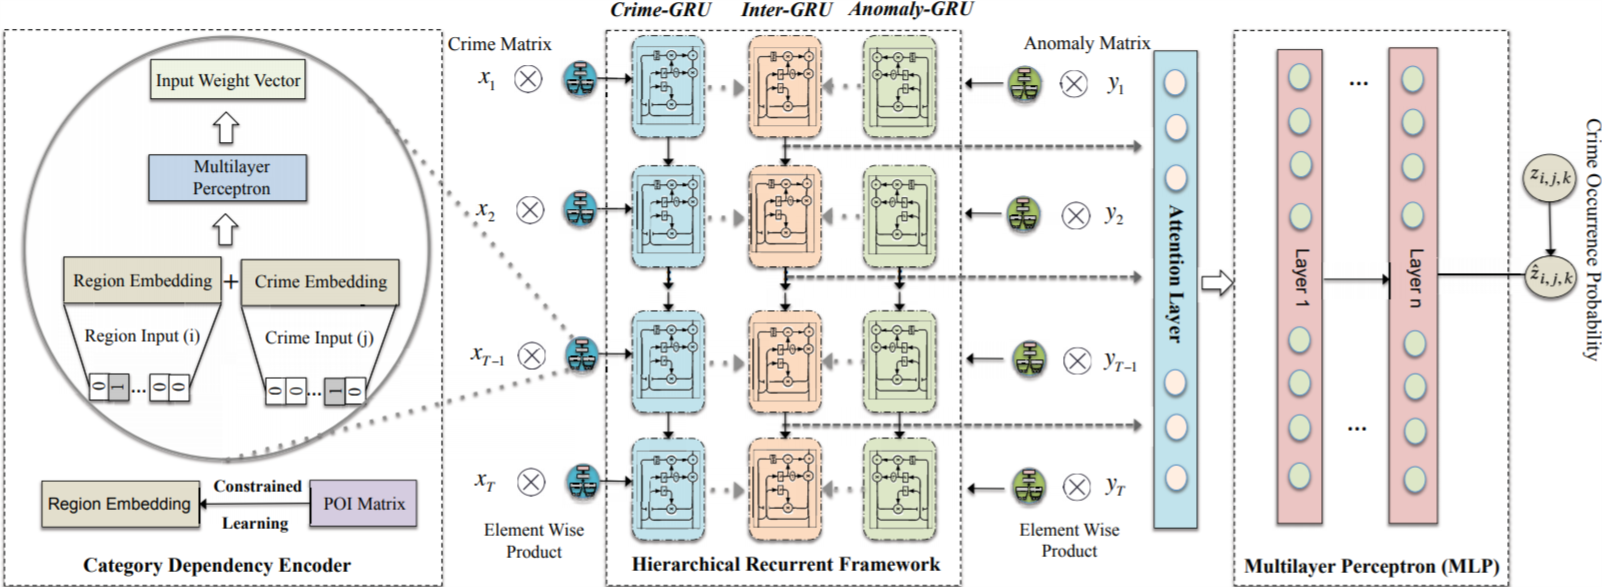
\includegraphics[width=.95\textwidth]{Chapter3/Plots_Chapter3/framework.png}
	\caption{The model architecture of the framework}
	\label{fig:framework}
	\end{center}
\end{figure}

In the third level, the aim is to employ another GRU encoder \emph{InterGRU} to model the inherent dependencies between the occurrence
of crimes and urban anomalies by concentrating their respective
hidden state from each time slot.

The corresponding hidden state in Crime-GRU, Anomaly-GRU and Inter-GRU, respectively are formally defined as follows:

\begin{align}
    h_t     &=      \text{GRU}(CM_i,h_{t-1})\notag\\
    g_t     &=      \text{GRU}(AM_i,g_{t-1})\notag\\
    \lambda_t &=    \text{GRU}(\Lambda,h_{t-1})
\end{align}
where $h_t$ and $g_t$ represent the hidden state corresponding to Crime-GRU and Anomaly-GRU encoder, respectively. In particular, we
feed a concatenated vector [$h_t$:$g_t$] as input into the Inter-GRU encoder to explore the dynamic interactions between the occurrences of crimes and urban anomalies. $\Lambda$ denotes the sequence of concatenated vector across $T$ time slots. \\Formally, $\Lambda = [[h_1:g_1],...,[h_T,g_T]]$. $\lambda_t$ is the hidden state of Inter-GRU encoder which captures the inherent dependencies between the crime and anomaly sequence.

\section{Attention Mechanism}

One limitation of the recurrent neural network based architectures
lies in that they encode the input sequence to a fixed length internal
representation, which results in worse performance for long input
sequences [25]. To overcome this limitation, the attention mechanism was proposed to allow the proposed hierarchical recurrent
framework to learn where to pay attention in the input sequence
for each item in the output sequence [29]. Particularly, the attention
mechanism aims to free the encoder-decoder architecture from the
fixed-length internal representation by introducing a context vector
to model the relevance. Formally, the attention mechanism can be
represented as follows:
\begin{align}
            u_m &= tanh(W_\nu\nu_m + b_\nu)\notag\\
            \alpha_m &= \frac{exp(W_uu_m)}{\sum_{m^{'}}exp(W_uu_{m^{'}})}\notag\\
            \hat{\nu} &= \sum_{m=1}^M\alpha_m\nu_m \label{eq3}
\end{align}
where we use $S$ to represent the attention dimension size. \(W_\nu \in R^{S\times R} \text{ and } W_u \in R^{1\times S}\) represent attention weight metrics. $b_m \in R^S$ is the attention bias. The number of input vectors is denoted by $M$. $\alpha_m$ m indicates the learned importance weight which corresponds to projected vector $\nu_m$ and $\hat{\nu}$ represents the new hidden representation which concatenates different hidden vectors. $W_u$ and $W_m$ are defined as two transmission matrices. For simplicity, Eq. \ref{eq3} is denoted as $\hat{\nu} = $ Attention($\nu_1,...,\nu_m,...,\nu_M$) in the following subsections. 

Our objective is to predict the crime occurrence in each region \(R_i \in [R_1,...,R_I]\) in the target time slot, based on the distribution
patterns of past crimes and urban anomalies, \emph{i.e.,} $[x_1,...,x_T]$ and $[y_1,...,y_T]$. However,the recurrent framework only encodes the input sequence from previous slots with a fixed length $T$ using internal representations and the performance will drop when the sequence length is large. To address this drawback, an attention mechanism is employed on the recurrent framework to
capture the relevance of crime patterns learned from previous time
slots in assisting the prediction of future crime occurrences.

In this attention mechanism, the importance of
anomaly occurrence in past time slots is estimated by deriving a normalized
importance weight via a softmax function. $\hat{\lambda}$ is defined as the concatenated hidden state in the attention mechanism as: $\hat{\lambda} = \text{Attention}(\lambda_1,...,\lambda_T)$.

\section{Multilayer Perceptron (MLP)}

Finally, the Multilayer Perceptron (MLP) component is utilized
to derive the occurrence probability by capturing the non-linear
dependencies between elements in hidden vectors. Formally, the MLP is represented as follows:
\begin{align}
            L_1 &= \phi(W_1 \cdot \lambda_1 + b_1)\notag\\
                &......\notag\\
            L_n &= \phi(W_n \cdot \lambda_n + b_n)\notag\\
            z_{i,j,k} &= \sigma(W^{'} \cdot L_n + b^{'})
\end{align}
where $n$ represents the number of hidden layers in MLP (indexed by $l$). For the $L_l$ layer, $W_l$ and $b_l$ represent the activation function
(i.e., \emph{ReLU} function) of MLP layers, weight matrix and bias vector,
respectively. The activation function is specified as sigmod (denoted as $\sigma$) to output the crime occurrence probability of category $C_j$ at region $R_i$ in \emph{k}-th time slot, \emph{i.e.,} $z_{i,j,k}$. In the experiments, the number of layers in MLP is set as 3.

\section{Learning Process}

In this subsection, learning process of the framework as introduced in Section 3, the objective is to derive the value of $z_{i,j,k}$ which denotes: does crime with category $C_j$ occur at region $R_i$ in \emph{k}-th time slot. A commonly used metric in the loss function of binary classification tasks is cross entropy [22]. Thus, the loss function which incorporates the constraint
term in Eq. \ref{1} is defined as follows:
\begin{align}
    L   &=  - \sum_{i,j,k} z_{i,j,k} \text{log}\hat{z}_{i,j,k} + (1 - z_{i,j,k}) \text{ log}(1 - \hat{z}_{i,j,k}) \notag \\
        &+  \frac{1}{R} | E_R - P_M \cdot W_{POI} |
\end{align}
where $\hat{z}_{i,j,k}$ denotes the estimated probability of \emph{j}-th category crime occurrence in region $R_i$ in \emph{k}-th time slot. Here, \emph{S} is the sampled crimes in the training process. The weights can be achieved by minimizing the loss function. In this work, Adaptive Moment
Estimation (Adam) [17] is used to learn the parameters of the framework.

% Buck \textendash boost converters allow to keep the bus voltage constant since any level of 
% string current can be set. Thus, the upper limit of PV panels per string for the buck\textendash boost 
% converter concept depends on the maximum output current rating, and the lower limit depends on the 
% maximum output voltage rating of the buck\textendash boost converters. In Table (\ref{table:max_minPVpanels}),
% the equations for the maximum and minimum numbers of PV panels per string are given for the 
% three different full\textendash power converter topologies under the assumption that all panels 
% should be able to feed power into the string under a given shading condition which can be 
% expressed as $\Delta = \frac{P_{PV,unsh}}{P_{PV,sh}}$ . 

% \begin{table}[h]
% 	\centering
% 		\begin{center}
% 		\centering
% 		\caption{Maximum, Resp. Minimum number of PV panels per string for different MIC topologies} \label{table:max_minPVpanels}
% 		\end{center}
% 	\centering
% 	\begin{tabular}{l|c|c}
% 	\hline \rule[-2ex]{0pt}{5.5ex} Type & Max. no. of PV panels & Min. no. of PV panels \\ \hline 
% 	\hline \rule[-2ex]{0pt}{5.5ex} 
%   	    Buck &$\frac{V_{BUS}}{P_{PV,MAX}}I_{OUT,MAX}$  & $(\frac{V_{BUS}}{V_{MPP}}\Delta +1$) \\ 
% 	\hline \rule[-2ex]{0pt}{5.5ex} 
% 	    Boost &$\frac{V_{BUS}+(\Delta-1)V_{MPP}}{\Delta.V_{MPP}}$  &$(\frac{V_{BUS}}{V_{out,MPP}}-1)\Delta+1$  \\ 
% 	\hline \rule[-2ex]{0pt}{5.5ex} 
% 	   Buck-Boost &$\frac{V_{BUS}}{P_{PV,MAX}}I_{OUT,MAX}$  & $(\frac{V_{BUS}}{V_{out,MPP}}-1)\Delta+1$ \\ 
% 	\hline 
% 	\end{tabular} 
% \end{table}

% Here, 
% \begin{enumerate}[(i)]
% 	\item $I_{Out,Max}$ is the maximum output current of the converter
% 	\item $V_{MPP}$ is the PV panel voltage in a typical MPP
% 	\item $P_{PV,max}$ is the the maximum output power
% \end{enumerate}



% \section{Giving references}
% An equation, figure or table given in any chapter can be called as follows: (For details refer the .tex file of this chapter). 

% Consider (\autoref{table:max_minPVpanels}) and (\autoref{fig:buckboost}) given in Chapter(\ref{chap:app}). Chapter reference can also be 
% given as (\autoref{chap:app}). 

% Citations can be given as \cite{a2}. Any reference to books can also be noted in the bib file and can be cited as \cite{b1} and proceedings in 
% the form \cite{p1}.


% \section{Matrix Equation}
% Matrices can be given as in equation (\ref{eq.matrixA}),
% \begin{eqnarray}
% 	\dot x = \mathbf Ax \label{eq.stateeqn}
% \end{eqnarray}

% where,
% \begin{eqnarray}
% 	\mathbf A = \begin{bmatrix}
% 	             a_1 & a_2 & a_3 \\
% 	             b_1 & b_2 & b_3 \\
% 	             c_1 & c_2 & c_3 \\
% 	      	    \end{bmatrix} \label{eq.matrixA}
% \end{eqnarray}


% \section{Figures}

% Figures can be grouped and separate captions can be given for each figure as Figure (\ref{fig:subcaption1}), (\ref{fig:subcaption2}) and (\ref{fig:subcaption3}). A caption can also be given for the group as Figure (\ref{fig:maincaption}). See the .tex file for details. 

% %Figure - 3D icosahedral quasicrystal- Al-Pd-Mn
% %====================================
% \begin{figure}
%     \centering
%     \begin{subfigure}[b]{0.48\textwidth}
%         \centering
%         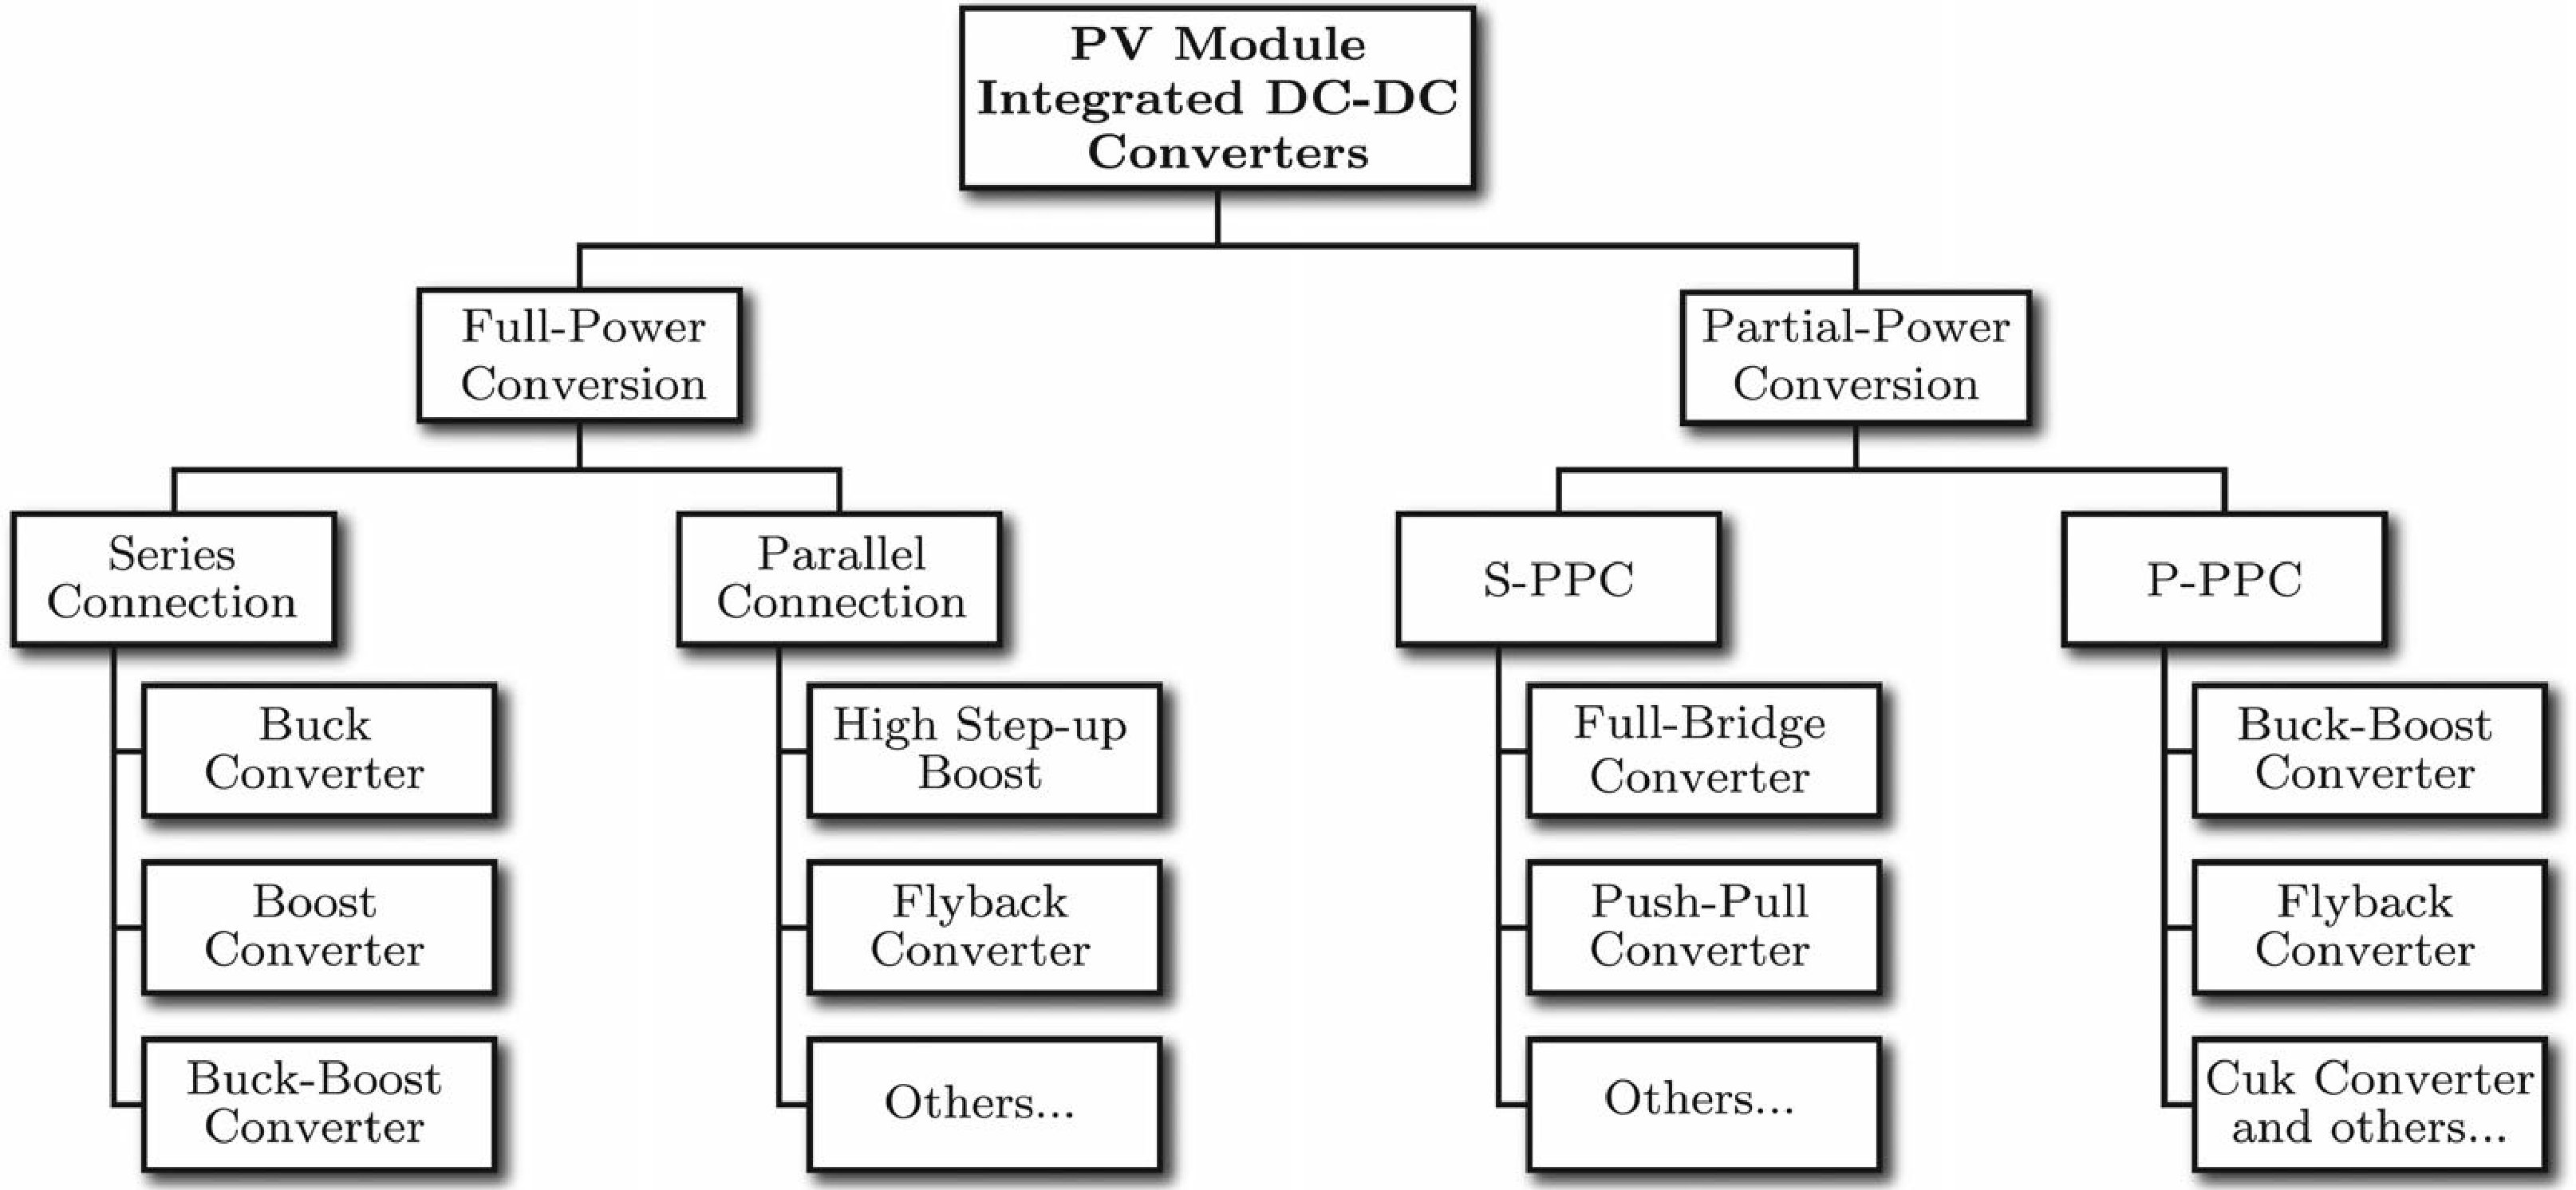
\includegraphics[width=\textwidth, height=0.75\textwidth]{Chapter3/Plots_Chapter3/fig2.pdf}
%         \caption{Subcaption 1}
%         \label{fig:subcaption1}
%     \end{subfigure}
%     \hfill
%     \begin{subfigure}[b]{0.48\textwidth}
%         \centering
%         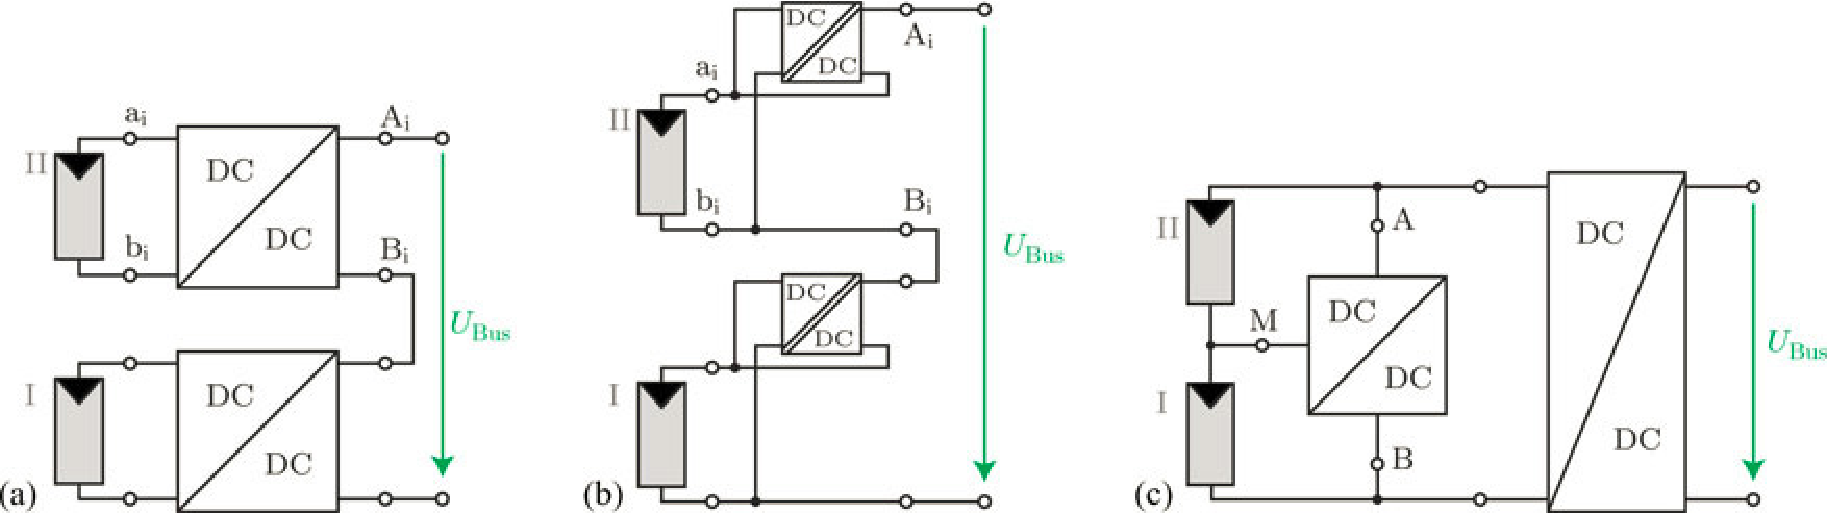
\includegraphics[width=\textwidth, height=0.75\textwidth]{Chapter3/Plots_Chapter3/fig3.pdf}
%         \caption{Subcaption 2}
%         \label{fig:subcaption2}
%     \end{subfigure}
%     \hfill
%     \begin{subfigure}[b]{0.48\textwidth}
%         \centering
%         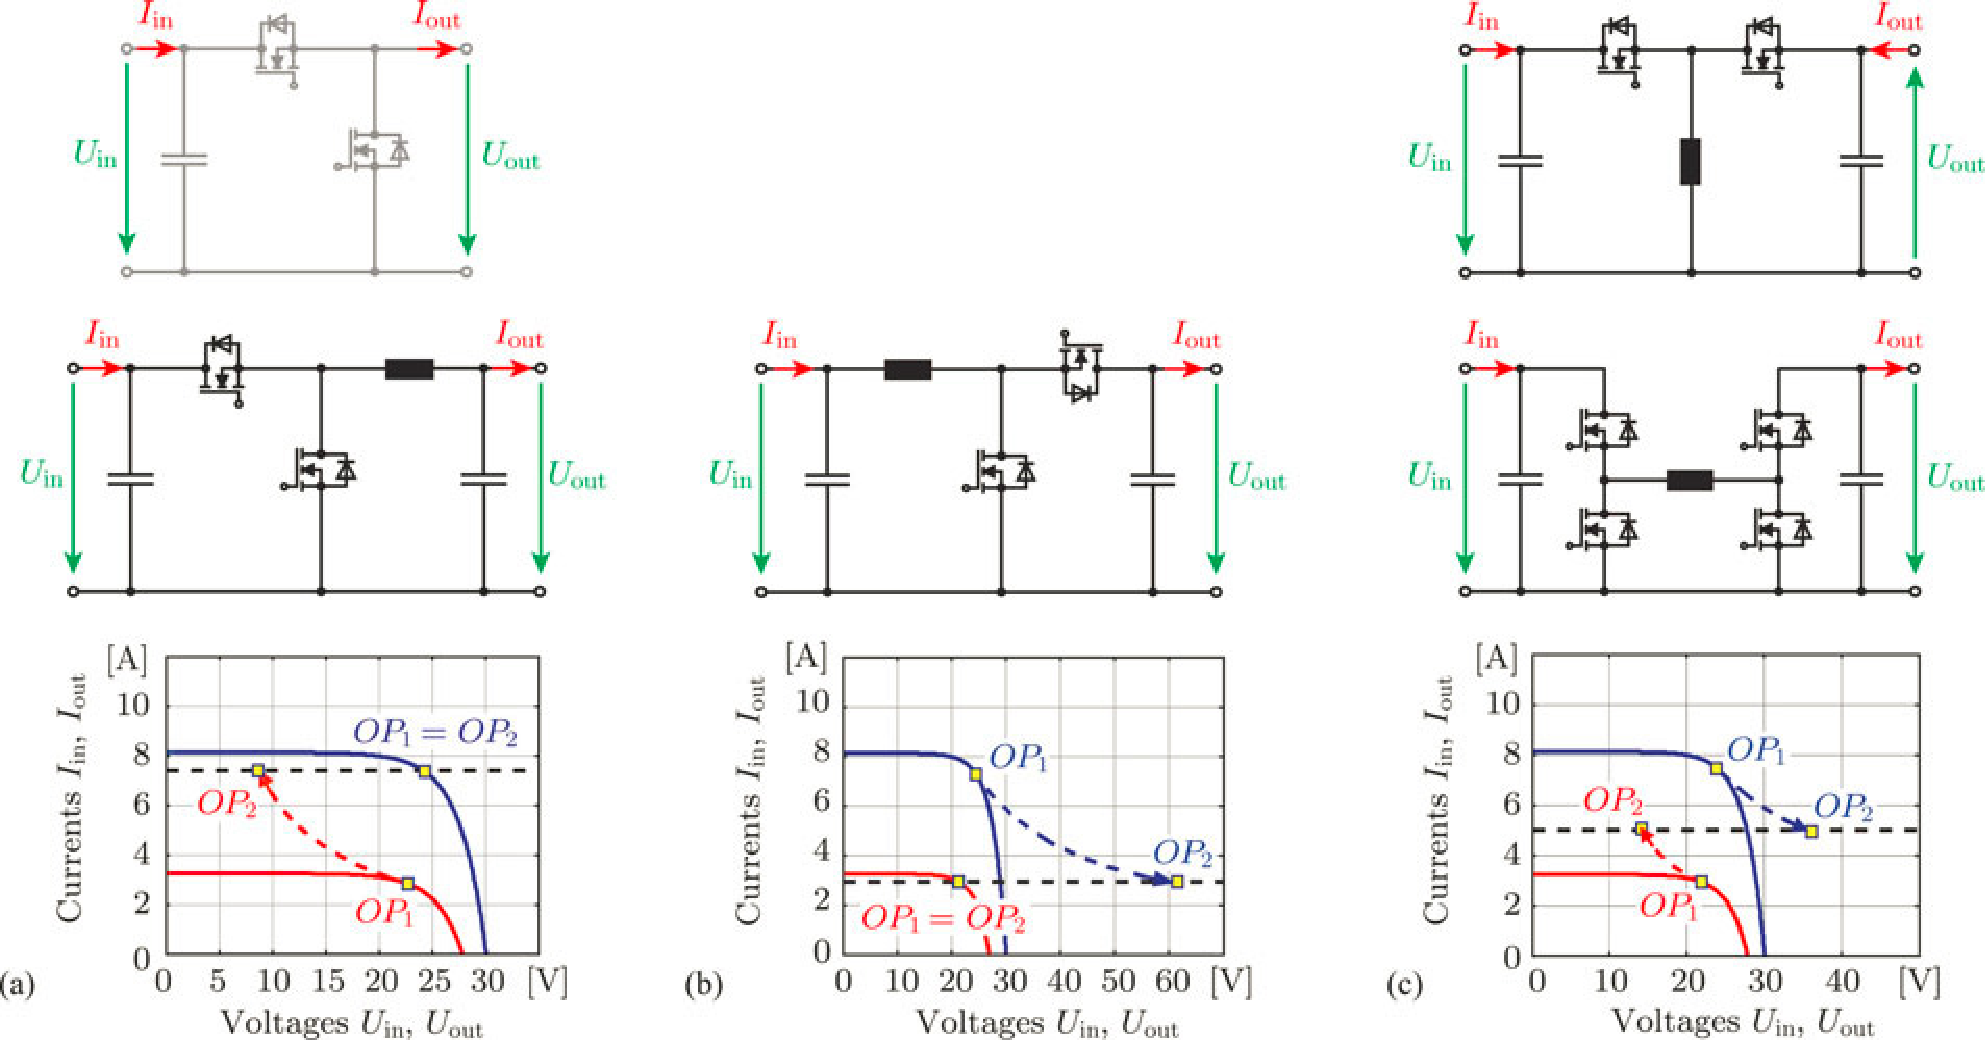
\includegraphics[width=\textwidth, height=0.75\textwidth]{Chapter3/Plots_Chapter3/fig4.pdf}
%         \caption{Subcaption 3}
%         \label{fig:subcaption3}
%     \end{subfigure}
%   \caption{Main caption}
%     \label{fig:maincaption}
% \end{figure}


